\documentclass{article}
\usepackage[utf8]{inputenc}
\usepackage{hyperref}
\usepackage[letterpaper, portrait, margin=1in]{geometry}
\usepackage{enumitem}
\usepackage{amsmath}
\usepackage{booktabs}
\usepackage{graphicx}
\usepackage{amsmath}

\usepackage{hyperref}
\hypersetup{
colorlinks=true,
    linkcolor=black,
    filecolor=black,      
    urlcolor=blue,
    citecolor=black,
}
\usepackage{natbib}

\usepackage{titlesec}
\titleformat{\section}
{\normalfont\Large\bfseries}{\thesection}{1em}{}[{\titlerule[0.8pt]}]


\title{ECON7103HW4}
\author{Sedat Ors}
\date{12 February 2024}

\begin{document}

\maketitle

\section{Python}
\vspace{0.5cm}
\begin{enumerate}
\item 
\noindent According to the Figure \ref{fig:question1} 1, there are parallel trends before treatment. 

\begin{figure}[ht]
    \centering
     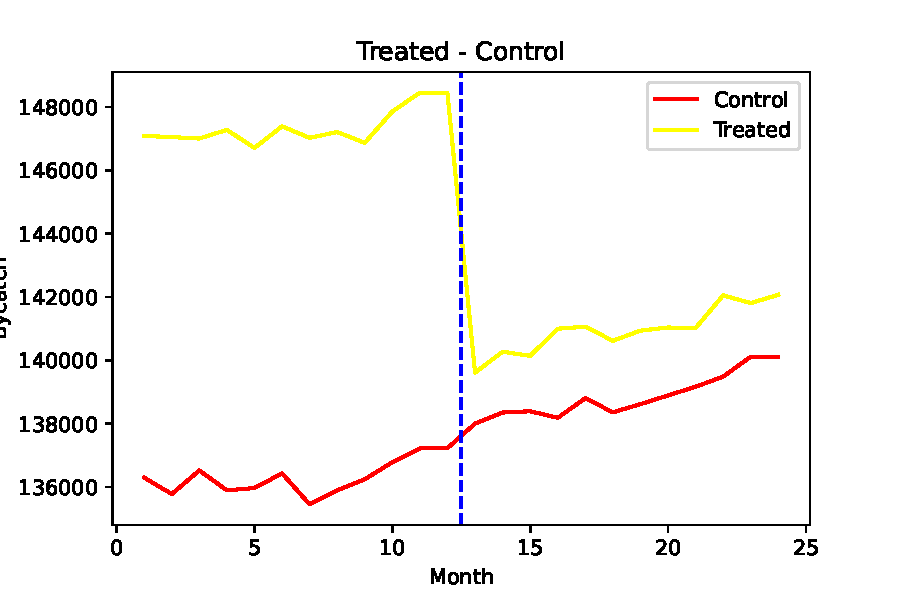
\includegraphics{hw4Q1.pdf}
    \caption{The figure indicates average firm bycatch in pounds for each month in 2017 and 2018}
    \label{fig:question1}
\end{figure}

\item The estimation is -9,591 which means that treatment leads decline in treatment group. 

\item
\noindent See Table \ref{tab:question3} 1 for results.
\vspace{0.5cm}
\begin{table}[ht]
    \centering
    \begin{tabular}{llll}
\toprule
{} &                     (1) &                    (2) &                   (3) \\
\midrule
Alpha           &               138001.81 &                    NaN &                   NaN \\
                &  (100507.57, 175496.06) &                    NaN &                   NaN \\
Pre period      &                 -773.22 &                    NaN &                   NaN \\
                &      (-1976.32, 429.89) &                    NaN &                   NaN \\
Treatment       &                11202.04 &                    NaN &                   NaN \\
                &   (-36028.81, 58432.89) &                    NaN &                   NaN \\
Time Treated    &                -9591.35 &                    NaN &                   NaN \\
                &   (-16085.87, -3096.83) &                    NaN &                   NaN \\
After-treatment &                   100.0 &                    NaN &                   NaN \\
Alpha           &                     NaN &              132088.04 &                   NaN \\
                &                     NaN &   (96407.7, 167768.38) &                   NaN \\
Treatment       &                     NaN &               11052.45 &                   NaN \\
                &                     NaN &  (-35515.12, 57620.02) &                   NaN \\
Time Treated    &                     NaN &               -8956.78 &                   NaN \\
 
After-Treatment &                     NaN &                 1200.0 &                   NaN \\
Alpha           &                     NaN &                    NaN &               1547.01 \\
                &                     NaN &                    NaN &    (-675.23, 3769.24) \\
Treatment       &                     NaN &                    NaN &                 -21.9 \\
                &                     NaN &                    NaN &     (-641.34, 597.54) \\
Time Treated    &                     NaN &                    NaN &              -8436.28 \\
                &                     NaN &                    NaN &  (-14111.27, -2761.3) \\
shrimp          &                     NaN &                    NaN &                  1.06 \\
                &                     NaN &                    NaN &          (0.95, 1.16) \\
salmon          &                     NaN &                    NaN &                   0.6 \\
                &                     NaN &                    NaN &          (0.18, 1.02) \\
firmsize        &                     NaN &                    NaN &              -2119.71 \\
 
\bottomrule
\end{tabular}

    \caption{Regression results with heteroskedasticity-robust standard errors.}
    \label{tab:question3}
\end{table}


\end{enumerate}

\section{Stata}
\vspace{0.5cm}
\begin{enumerate}
\item
\noindent See Table \ref{tab:quesion4}  2 for results.
\begin{table}[ht]
    \centering
    \documentclass[]{article}
\setlength{\pdfpagewidth}{8.5in} \setlength{\pdfpageheight}{11in}
\begin{document}
\begin{tabular}{lcc} \hline
 & (1) & (2) \\
VARIABLES & model1 & model2 \\ \hline
 &  &  \\
shrimp & 1.500*** &  \\
 & (0.0708) &  \\
salmon & -2.323*** &  \\
 & (0.220) &  \\
shrimp\_demean &  & 1.540*** \\
 &  & (0.0672) \\
salmon\_demean &  & 1.598*** \\
 &  & (0.444) \\
treated\_demean &  & 640,873*** \\
 &  & (39,088) \\
Constant & 366,278*** & -259,368*** \\
 & (30,113) & (29,480) \\
 &  &  \\
Observations & 1,200 & 1,200 \\
R-squared & 0.286 & 0.400 \\
 Number of firm & 50 & 50 \\ \hline
\multicolumn{3}{c}{ Standard errors in parentheses} \\
\multicolumn{3}{c}{ *** p$<$0.01, ** p$<$0.05, * p$<$0.1} \\
\end{tabular}
\end{document}

    \caption{Stata Results}
    \label{tab:quesion4}
\end{table}

\end{enumerate}

\end{document}
